\documentclass[12pt]{article}
\usepackage[top=1in, bottom=1in, left=1in, right=1in]{geometry}
\usepackage[justification=centering]{caption}
\usepackage{graphicx}
\usepackage{listings}
\usepackage{color}
\usepackage{indentfirst}
\usepackage{hyperref}
\usepackage{siunitx}
\usepackage{float}
\usepackage{amsmath}

\lstset{ %
	%language=C,                % choose the language of the code
	basicstyle=\scriptsize,       % the size of the fonts that are used for the code
	                  % how far the line-numbers are from the code
	backgroundcolor=\color{white},  % choose the background color. You must add \usepackage{color}
	showspaces=false,               % show spaces adding particular underscores
	showstringspaces=false,         % underline spaces within strings
	showtabs=false,                 % show tabs within strings adding particular underscores
	%frame=single,           % adds a frame around the code
	tabsize=2,          % sets default tabsize to 2 spaces
	captionpos=b,           % sets the caption-position to bottom
	breaklines=true,        % sets automatic line breaking
	breakatwhitespace=false,    % sets if automatic breaks should only happen at whitespace
	escapeinside={\%*}{*)}          % if you want to add a comment within your code
}

\begin{document}
\title{Microprocessor Systems\\ Lab 6: Memory Interfacing }
\author{Nick Choi \and Samuel Deslandes}
\date{12/05/16}
\maketitle
\pagebreak
\section{Introduction}


\section{Methods}
\subsection{Software}
The code for parts 1, 2 and 3 can be found in Appendix A, B and C respectively. All code was uploaded and run on the 8051 through the programming/debugging USB port. 

\subsubsection{Part 1}
In the first section of this lab an electronic ``Magic 8 Ball'' was developed. The program generates responses to four types of questions that can be asked:
	\begin{itemize}
		\item Yes/No
		\item True/False
		\item Day of the week
		\item Random Number
	\end{itemize}

In order to randomly select a response, Timer0 is is configured to continuously count, and is sampled when a response is required. Timer0 was configured as a 16-bit timer by setting the lower nibble of the TMOD SFR to \texttt{0x01}. Although Timer0 is a 16-bit timer, only the lower byte (stored in TL0) is sampled. The timer was also configured to use SYSCLK/12 as a base by clearing bits 0, 1, and 3 of the CKCON SFR. 

When configuring ports, bits 0--3 of port 3 should be configured as inputs, and bits 4--7 as outputs. This is done by setting the `P3MDOUT' SFR to \texttt{0xf0}, and the `P3' SFR to \texttt{0x0F}.

In the main function, user input is retrieved using the getchar() function. A switch/case block is then used to handle the user input and generate the appropriate response. In the case of a binary response, such as for the `Yes/No' or `True/False' questions, TL0 is read and modded by 2. The result is then evaluated to be either 1 or 0 and a response is printed to the terminal accordingly. 

To handle the `Days of the week' question an array of strings declared as ``const char*'' was used to store each day of the week. The value held in TL0 is then modded by 7 and used to index the aforementioned array. In order to print the string, `printf()' was used with the `\%s' formatting keyword. 

To handle the `Random number' question case, first the user must be prompted for max and min values to designate a range of responses. This is done using `getchar()'. To randomly select an integer within this range the following equation is used:
\begin{displaymath}
\text{min+TL0\%(max-min+1)}
\end{displaymath}
The right side of the equation produces a number within the difference of the max and min values selected; adding the minimum value to this brings it back within the range. 

In addition to the four cases corresponding to the types of questions that can be asked, there is also the default case, which is triggered when the input is invalid. In this case the program notifies the user of the invalid input and waits for the next user input. 

\subsubsection{Part 2}
The code for this section of the lab is an enhancement of the previous part, which prints output not only to the terminal, but also to an LCD screen. In order to print to the LCD screen, first the ``LCD.h'' and ``LCD.c'' files must be included; these files contain the functions ``lcd\textunderscore clear()'' and ``lcd\textunderscore puts()'' which are used to clear the LCD and write to the LCD respectively, as well as the ``lcd\_init()'' function used to initialize the LCD. As mentioned before, the code for this section is the same as that of the previous section, with the addition of the ``lcd\_init()'' function called together with the other init functions, and clearing the LCD and printing to it after printing to the terminal when outputting responses. 

\subsubsection{Part 3}
The code for this section further enhances that of the previous section by using a keypad to receive user input, rather than the keyboard. The keypad is wired such that when a key is pressed, an external interrupt (/INT0) is triggered. To do this, /INT0 must be routed to port pin P0.2, which is done by setting bit 2 of the XBR1 SFR. Next, global interrupts and /INT0 must be enabled, which can be done using the bit-addressable variables `EA' and `EX0' respectively. 

%talk about key wakeup and decoding

\subsection{Hardware}

\subsubsection{Part 1}

\subsubsection{Part 2}

\subsubsection{Part 3}

\section{Results}



\section{Conclusion}
 


\section{Appendices}
\subsection{Modified putget.h}
\lstinputlisting{putget.h}

\subsection{Part 1}
\subsubsection{Code}
	\lstinputlisting{part1.c}
\subsection{Part 2}
\subsubsection{LCD Schematic}
\begin{figure}[H]
	\centering
	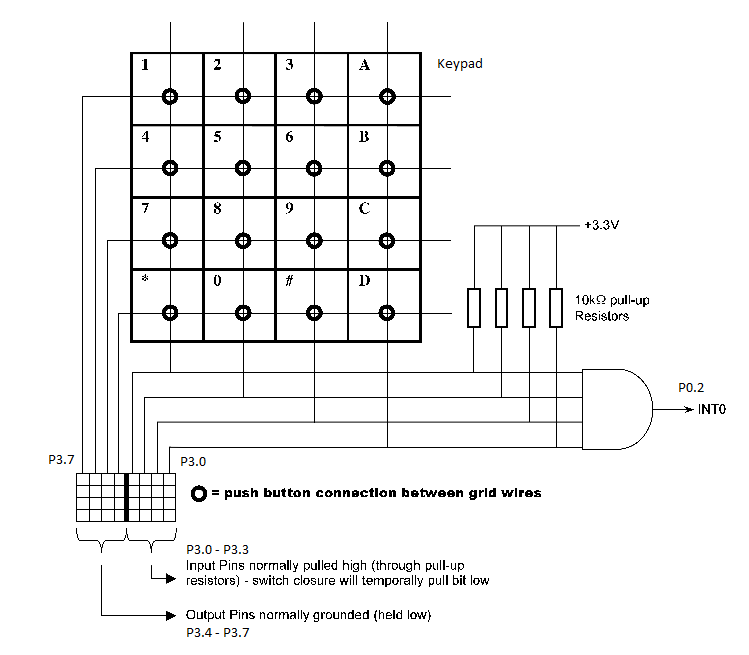
\includegraphics[width=\textwidth]{keypad_schematic.png}
	\caption{Circuit schematic for LCD}
	\label{LCD}
\end{figure}

\subsubsection{Code}
	\lstinputlisting{part2.c}	
\subsection{Part 3}
\subsubsection{Keypad Schematic}
\begin{figure}[H]
	\centering
	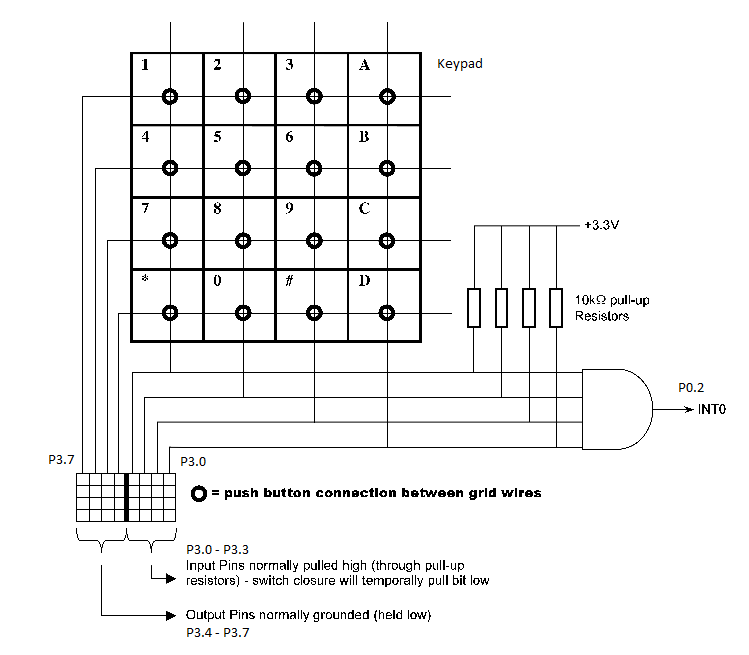
\includegraphics[width=\textwidth]{keypad_schematic.png}
	\caption{Circuit schematic for keypad}
	\label{KEY}
\end{figure}
\subsubsection{Code}
	\lstinputlisting{part3.c}

\section{References} 
\noindent
``MPS Lab 6," in RPI ECSE Department, 2016. [Online]. Available: \url{http://www.rpi.edu/dept/ecse/mps/MPS_Lab_Ex5-Memory.pdf}. Accessed: Nov. 27, 2016.\\
\newline\noindent
``C8051 Manual," in RPI ECSE Department, 1.4 ed., 2005. [Online]. Available: \url{https://www.ecse.rpi.edu/courses/CStudio/Silabs/C8051F12x-13x.pdf}. Accessed: Nov. 27, 2016.


\end{document}